 
\documentclass{beamer}
\usepackage{indentfirst}
\usepackage{amsmath,amssymb,amsthm,amsbsy,amsfonts,amsxtra,mathabx,amscd}
\usepackage{wrapfig}
\usepackage{graphicx}
\usepackage{graphics,graphpap}
\usepackage{xcolor}
\usepackage{subfig}
\usepackage{caption}
\usepackage{url}
\usepackage{upgreek}
\usepackage{mathtools}
\usepackage{calc}
\usepackage{slashed}
\usepackage{mathrsfs}

\newtheorem{thm}{Theorem}[section]
\newtheorem{cor}[thm]{Corollary}
\newtheorem{lem}[thm]{Lemma}
\newtheorem{prop}[thm]{Proposition}
\newtheorem{prob}[thm]{Problem}

\newenvironment{soln}{\renewcommand{\proofname}{Solution}\begin{proof}}{\end{proof}}

\theoremstyle{definition}
\newtheorem{rem}{Remark}[section]
\newtheorem{obs}{Observations}[section]
\newtheorem{defin}{Definition}[section]
\newtheorem{res}{Result}[section]
\newtheorem{eg}{Example}[section]
\newtheorem{egs}{Examples}[section]
\newtheorem{case}{Case}
\newtheorem*{notn}{Notation}
\makeatletter\@addtoreset{case}{thm}\makeatother
\usepackage[T1]{fontenc}
\usepackage{pstricks}
\usepackage{pst-3dplot}


\usepackage{tikz}
\usetikzlibrary{matrix}
\usepackage{tkz-euclide,tkz-fct}
\usepackage{tikz-cd}
\usetikzlibrary{arrows}
\usetikzlibrary{calc,fadings,decorations.pathreplacing}
\usepackage{tqft}
\usepackage{pgfplots}

\usepackage[all,2cell]{xy}
\UseAllTwocells

\usepackage{enumerate}
\usepackage{enumitem}

\usepackage{bookmark}


\usepackage{verbatim}
\usepackage{float}

\usepackage{mfirstuc}

\makeatletter
\newcommand{\BH}[1]{\hyperpage{#1}\normalsize}
\newcommand{\define}[1]{%
	\textbf{#1}%
	\index{#1|BH}%
}
\makeatother

\DeclareMathOperator{\ob}{ob}
\DeclareMathOperator{\Hom}{Hom}
\DeclareMathOperator{\id}{id}
\DeclareMathOperator{\End}{End}
\DeclareMathOperator{\dvol}{dvol}
\DeclareMathOperator{\coker}{coker}
\DeclareMathOperator{\Cas}{Cas}
\DeclareMathOperator{\Id}{Id}


% There are many different themes available for Beamer. A comprehensive
% list with examples is given here:
% http://deic.uab.es/~iblanes/beamer_gallery/index_by_theme.html
% You can uncomment the themes below if you would like to use a different
% one:
\usetheme{metropolis}
%\usetheme{AnnArbor}
%\usetheme{Antibes}
%\usetheme{Bergen}
%\usetheme{Berkeley}
%\usetheme{Berlin}
%\usetheme{Boadilla}
%\usetheme{boxes}
%\usetheme{CambridgeUS}
%\usetheme{Copenhagen}
%\usetheme{Darmstadt}
%\usetheme{default}
%\usetheme{Frankfurt}
%\usetheme{Goettingen}
%\usetheme{Hannover}
%\usetheme{Ilmenau}
%\usetheme{JuanLesPins}
%\usetheme{Luebeck}
%\usetheme{Madrid}
%\usetheme{Malmoe}
%\usetheme{Marburg}
%\usetheme{Montpellier}
%\usetheme{PaloAlto}
%\usetheme{Pittsburgh}
%\usetheme{Rochester}
%\usetheme{Singapore}
%\usetheme{Szeged}
%\usetheme{Warsaw}

\titlegraphic{%
	\begin{picture}(0,0)
		\put(335.8,22.8){\makebox(0,0)[rt]{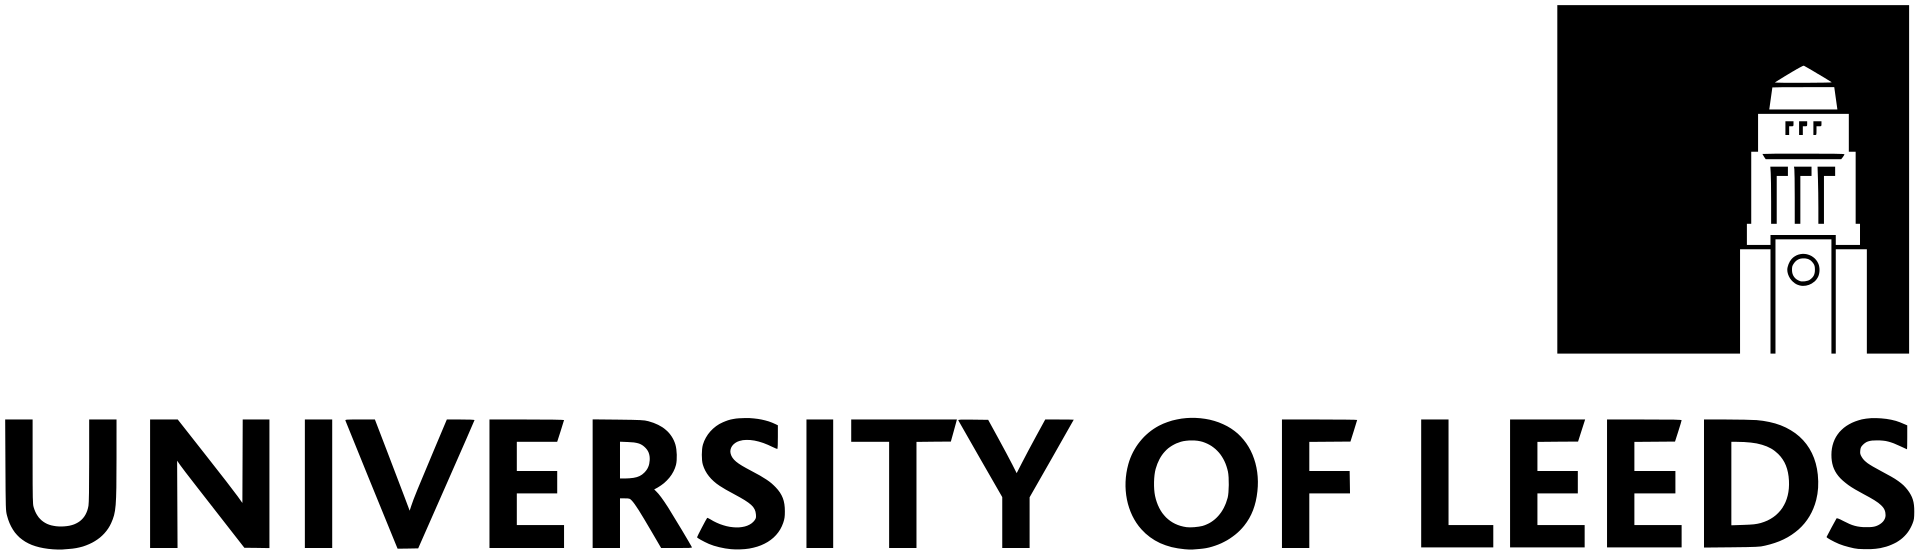
\includegraphics[width=4.5cm]{logo.png}}}
\end{picture}}
\title{\bf An Introduction to Instantons \\in Higher Dimensions}

% A subtitle is optional and this may be deleted
%\subtitle{A Journey Towards $4$ Manifolds}

\author{Tathagata Ghosh\inst{}}
% - Give the names in the same order as the appear in the paper.
% - Use the \inst{?} command only if the authors have different
%   affiliation.

\institute[University of Leeds] % (optional, but mostly needed)
{
	\inst{}%
	School of Mathematics\\
	University of Leeds
}\date{July 21, 2022}
% - Use the \inst command only if there are several affiliations.
% - Keep it simple, no one is interested in your street address.

\date{School of Mathematics Postgraduate Research Conference, \\
University of Leeds, June 15--17, 2022}
% - Either use conference name or its abbreviation.
% - Not really informative to the audience, more for people (including
%   yourself) who are reading the slides online

%\subject{An Introduction to Instantons in Higher Dimensions}
% This is only inserted into the PDF information catalog. Can be left
% out. 

% If you have a file called "university-logo-filename.xxx", where xxx
% is a graphic format that can be processed by latex or pdflatex,
% resp., then you can add a logo as follows:

% \pgfdeclareimage[height=0.5cm]{university-logo}{university-logo-filename}
% \logo{\pgfuseimage{university-logo}}

% Delete this, if you do not want the table of contents to pop up at
\setbeamertemplate{section in toc}{\vspace*{-1em}\hspace*{1em}\inserttocsectionnumber.~\inserttocsection\par}
\setbeamertemplate{subsection in toc}{\vspace*{-0.5em}\hspace*{2em}\inserttocsectionnumber.\inserttocsubsectionnumber.~\inserttocsubsection\par}
% the beginning of each subsection:
\AtBeginSubsection[]
{
	\begin{frame}<beamer>{Outline}
		\vskip20pt
		\tableofcontents[currentsection,currentsubsection]
	\end{frame}
}

\begin{document}
	
	\begin{frame}
		\titlepage
	\end{frame}
	
	\begin{frame}{Outline}
		\vskip20pt
		\tableofcontents
		% You might wish to add the option [pausesections]
	\end{frame}
	
	% Section and subsections will appear in the presentation overview
	% and table of contents.
	
	\section{Introduction}
	\section{Introduction2}
	\begin{frame}{Introduction}{}
		\begin{itemize}
		    \item<1-> {Instantons are solutions of certain equations called instanton equations (duh!). They also solve the Yang--Mills equations.}
			\item<2-> {In 1862 James Clerk Maxwell came up with the electromagnetism equations, which unified the electric fields and magnetic fields. \uncover<3->{\begin{figure}\centering
						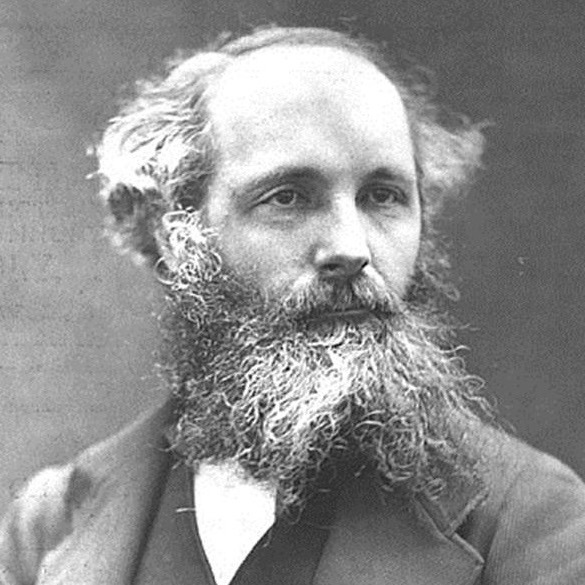
\includegraphics[scale=0.2]{Maxwell.jpg}\\
						James Clerk Maxwell
				\end{figure}}
			}
		\end{itemize}
	\end{frame}
	\begin{frame}{Introduction}{}
		\begin{itemize}
			\item<1-> {In 1954 Yang--Mills equations appeared as a generalization of Maxwell's theory. \uncover<2->{\begin{figure}\centering
						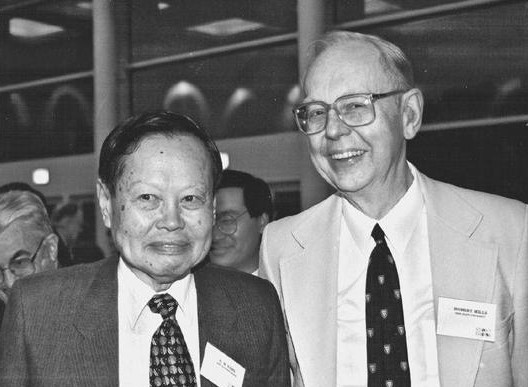
\includegraphics[scale=0.28]{Yang-Mills.jpg}\\
						Yang Chen-Ning and Robert Mills
				\end{figure}}
			}
			\item<3-> {Since then, the Yang--Mills theory in $4$-dimensions have been studied extensively by physicists and mathematicians alike.}
		\end{itemize}
	\end{frame}

	\section{Differential Forms}
	\begin{frame}{Differential Forms}{}
		\begin{itemize}
            \item<1-> {To describe the Yang--Mills equations and Instantons, we start with the notion of differential forms.}
            \item<2-> {Suppose we are in the Euclidean space $\mathbb{R}^3$. Denote a point by $(x, y, z)$ (or, $(x_1, x_2, x_3)$). We call $x, y, z$ coordinate functions. Now, we consider the `line elements' $dx, dy, dz$.}
            \item<3-> {This should be familier to you, since in one dimension $\mathbb{R}$, you have integrated a function $f(x)$ over some interval $[a, b]$ as $\int_a^b f(x)\ dx$.}
            \item<4-> {In two dimensions $\mathbb{R}^2$, you have integrated a function $f(x, y)$ over some region $R \subset \mathbb{R}^2$:
            $$\iint_R f(x, y)\ dxdy$$
            We called $dxdy$ the `area element'.}
        \end{itemize}
	\end{frame}
	\begin{frame}{Differential Forms}{}
		\begin{itemize}
            \item<1-> {Now, let's think of $dx, dy$ being vectors, having directions. If we take $dx$ first, then $dy$, the area element $dxdy$ has normal vector (which is $dx \times dy$) upwards, by thumb rule.\uncover<2->{\begin{figure}\centering
						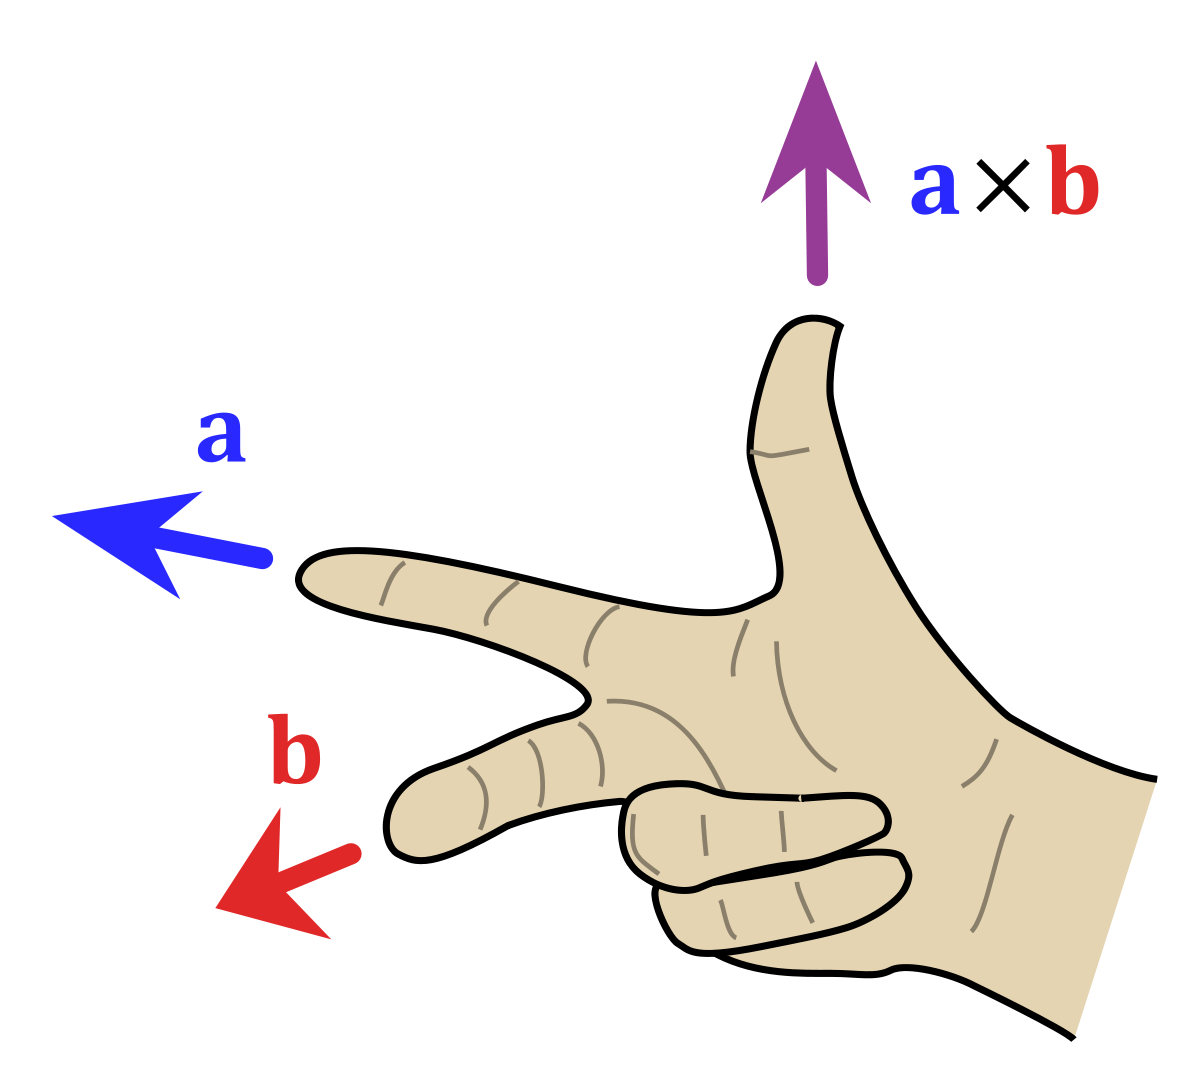
\includegraphics[scale=0.07]{thumb.png}
				\end{figure}}}
            \item<3-> {Now, if we take $dy$ first then $dx$, the area element $dydx$ has a normal vector ($dy \times dx$) is downwards, opposite to the previous one.}
            
        \end{itemize}
	\end{frame}
	\begin{frame}{Differential Forms}{}
		\begin{itemize}
		    \item<1-> {To incorporate this skew symmetry of the area element $dxdy$ (which is due to the issue of `orientation'), we denote $dxdy$ by
            $$dx \wedge dy$$}
            \item<2-> {$\wedge$ is called wedge product.}
            \item<3-> {Clearly, $dx \wedge dy = -dy \wedge dx$.}
            \item<4-> {Similarly, we have the volume element $dx \wedge dy \wedge dz$.}
        \end{itemize}
	\end{frame}
	\begin{frame}{Differential Forms}{}
		\begin{itemize}
            \item<1-> {Let we are still in $\mathbb{R}^3$, we call $x, y, z$ or any real valued function a $0$-form. We call $dx, dy, dz$ $1$-forms, $dx \wedge dy, dy \wedge dz, dz \wedge dx$ $2$-forms, and $dx \wedge dy \wedge dz$ a $3$-form. Clearly you can generalize this to any dimensions, for $\mathbb{R}^n$.}
            \item<2-> {These forms are linearly independent and spans vector spaces (Actually modules, being over (non-commutative) ring of all smooth real valued functions, $\Omega^0(\mathbb{R}^3)$).}
            \item<3-> {$dx, dy, dz$ spans $\Omega^1(\mathbb{R}^3) \cong \mathbb{R}^3$, the space of all $1$-forms.}
            \item<4-> {$dx \wedge dy, dy \wedge dz, dz \wedge dx$ spans $\Omega^2(\mathbb{R}^3)$, the space of all $2$-forms.}
            \item<5-> {$dx \wedge dy \wedge dz$ spans $\Omega^3(\mathbb{R}^3)$, the space of all $3$-forms.}
            \item<6-> {Note that in dimensions $3$, any $4$-form is zero (just like the volume of a plane object is zero).}
        \end{itemize}
	\end{frame}
	\begin{frame}{Differential Forms}{}
		\begin{itemize}
            \item<1-> {Any $1$-form on $\mathbb{R}^3$ can be written as $fdx + gdy + hdz$, for real valued functions $f, g, h \in \Omega^0$. any $2$ form can be written as $fdx \wedge dy + g dy \wedge dz + h dz \wedge dx$ etc.}
            \item<2-> {Before moving forward, we should mention that the `differential' $d$ of a $k$-form makes it a $k+1$-form.}
            \item<3-> {Simple example, $x$ is a $0$-form whereas $dx$ is $1$-form. }
            \item<4-> {Another one: $xdy\wedge dz$ is $2$-form but $d(xdy\wedge dz) = dx \wedge dy \wedge dz$ is $3$-form.}
            \item<5-> {Important note: $d^2 = 0$.}
        \end{itemize}
	\end{frame}
	\subsection{Hodge Star Operator}
	\begin{frame}{Hodge Star Operator}{}
		\begin{itemize}
            \item<1-> {We are still in $\mathbb{R}^3$. Recall the volume form $dx \wedge dy \wedge dz$. Hodge star of a form is the rest of the terms in the volume form. So, 
            $$*dx = dy \wedge dz$$
            Since, $dx \wedge dy \wedge dz = -dy \wedge dx \wedge dz$,
            $$*dy = -dx \wedge dz = dz \wedge dx$$
            $$*(dx \wedge dy) = dz\ \ \text{etc.}$$.}
            \item<2-> {Using the Hodge star, we define the `codifferential' $d^*$ which decreases forms. Define
            $$d^* = *d*$$}
        \end{itemize}
	\end{frame}
	\begin{frame}{Hodge Star Operator}{}
		\begin{itemize}
            \item<1-> {Then, in $3$-dimensions, for a $2$-form $F$, 
            \begin{align*}
                F &\in \Omega^2\\
                *F &\in \Omega^{3-2} = \Omega^1\\
                d*F &\in \Omega^{3-1} = \Omega^2\\
                *d*F &\in \Omega^{3-2} = \Omega^1
\end{align*}}
            \item<2-> {So,$d^* : \Omega^2 \to \Omega^1$ whereas $d : \Omega^1 \to \Omega^2$.}
            \item<3-> {Historically, Hodge introduced the star operator precisely to write down the Maxwell's equations in easier manner. So, let's do that now.}
        \end{itemize}
	\end{frame}
	\section{Maxwell's Equations}
	\begin{frame}{Maxwell's Equations}{}
		\begin{itemize}
            \item<1-> {In $\mathbb{R}^3$, the electric field $\mathbf{E} \in \Omega^1(\mathbb{R}^3)$ is a $1$-form and the magnetic field $\mathbf{B} \in \Omega^2(\mathbb{R}^3)$ is a $2$-form. Let $dx^1, dx^2, dx^3$ spans $\Omega^1(\mathbb{R}^3)$. Introduce the $4$th coordinate $t = x^0$, and so, $dt (= dx^0), dx^1, dx^2, dx^3$ spans $\Omega^1(\mathbb{R}^4)$.}
            \item<2-> {The Electromagnetic field (strength) is a $2$-form on space-time $\mathbb{R}^4$,
            $$\mathbf{F} = \mathbf{B} + dt \wedge \mathbf{E} \in \Omega^2(\mathbb{R}^4)$$
            We can write
            $$\mathbf{F} = \sum\limits_{0 \leq \mu , \nu \leq 3} F_{\mu\nu}dx^\mu \wedge dx^\nu.$$}
            \item<3-> {Now, we have
            $$d\mathbf{F} = 0$$
            which is Bianchi identity, it always holds. }
        \end{itemize}
	\end{frame}
	\begin{frame}{Maxwell's Equations}{}
		\begin{itemize}
            \item<1-> {Since $d^2 = 0$, we have an $1$-form $\mathbf{A} \in \Omega^1(\mathbb{R}^4)$ such that
        $$\mathbf{F} = d\mathbf{A}$$
        called the electromagnetic potential in space-time.}
            \item<2-> {Mathematicians usually call $\mathbf{A}$ the connection $1$-form and $\mathbf{F}$ the curvature $2$-form.}
            \item<3-> {The Maxwell's equations (in vacuum) in space-time are 
            \begin{align*}
            d\mathbf{F} &= 0\\
            d^*\mathbf{F} &= 0.
\end{align*}}
        \end{itemize}
	\end{frame}
	\section{Yang--Mills Equations}
    \begin{frame}{Yang--Mills Equations}{}
		\begin{itemize}
            \item<1-> {The connection $1$-form (or, electromagnetic potential) is real valued (we can think of it as a function $A : \mathbb{R}^4 \to \mathbb{R}$). So, for $x, y \in \mathbb{R}^4$,
            $$[A, A](x, y) := A(x)A(y) - A(y)A(x) = 0$$
            since for real numbers $a, b$ we have $ab = ba$ (i.e, commutativity).}
            \item<2-> {We can think of Yang--Mills equations as generalisations of Maxwell's equations where we consider the potential to $2 \times 2$ trace-less skew-Hermitian matrix valued function (rather than real i.e., $1 \times 1$ matrix-valued). Now, because of non-commutativity of matrices, in general,
            $$[A, A](x, y) := A(x)A(y) - A(y)A(x) \neq 0$$}
        \end{itemize}
	\end{frame}
	\begin{frame}{Yang--Mills Equations}{}
		\begin{itemize}
            \item<1-> {In this general setup, the curvature takes the form
            $$F_A = dA + [A,A]$$}
            \item<2-> {Define the covariant derivative
            $$d_A = d + [A, \cdot\ ]$$}
            \item<3-> {Then, $$F_A = d_AA$$
            (We should note that because of the extra term, $d_A^2$ is not in general zero.)}
            \item<4-> {Fianlly, we have the equations
            \begin{align*}
                d_AF_A &= 0\ \ \text{(Bianchi identity)}\\
                d_A^*F_A &= 0\ \ \text{(Yang--Mills equation)}
            \end{align*}}
        \end{itemize}
	\end{frame}
	\section{Finally, Instantons (in $4$-dimensions)}
	\begin{frame}{Instantons in $4$-dimensions}{}
		\begin{itemize}
            \item<1-> {We are in $4$-diemensional Euclidean space. Let's look at two particular equations
            \begin{align*}
            *F_A &= F_A\ \ \text{(Self-dual Instanton equation)}\\
            *F_A &= -F_A\ \ \text{(Anti-self-dual Instanton equation)}
            \end{align*}}
            \item<2-> {Dimensionally it makes sense, since $F_A \in \Omega^2 \Rightarrow *F_A \in \Omega^{4-2} = \Omega^2 \ni \pm F_A$.}
            \item<3-> {The solutions for these equations are the connections for which the curvature satisfies these equations. These connections are called Instantons.}
        \end{itemize}
	\end{frame}
	\begin{frame}{Instantons in $4$-dimensions}{}
		\begin{itemize}
            \item<1-> {Now,
            \begin{align*}
            d_A^*F_A &= *d_A*f_A\\
             &= d_A(\pm F_A)\ \ (\text{using instanton equations})\\
             &= \pm *d_AF_A\\
         &= 0\ \ (\text{using Bianchi identity})
        \end{align*}}
            \item<2-> {So, we see that instantons are indeed solutions of the Yang--Mills equations.}
        \end{itemize}
	\end{frame}
	
    \section{Instantons in higher Dimensions}
    \begin{frame}{Instantons in higher Dimensions}{}
		\begin{itemize}
            \item<1-> {Now, we want to do the same thing on $\mathbb{R}^7$. Here $F_A \in \Omega^2(\mathbb{R}^7)$. But then,\\
            $F_A \in \Omega^2 \Rightarrow *F_A \in \Omega^{7-2} = \Omega^5 \not\ni \pm F_A$. }
            \item<2-> {So, consider a $3$-form $\phi \in \Omega^3$,
            $$\phi = dx^1 \wedge dx^2\wedge dx^7 + dx^3 \wedge dx^4 \wedge dx^7 +  \dots$$}
            \item<3-> {Indeed,
            \begin{align*}
            &F_A \in \Omega^2\\
            &\phi \wedge F_A \in \Omega^{3+2} = \Omega^5\\
            &*(\phi \wedge F_A) \in \Omega^{7-5} = \Omega^2 \ni \pm F_A
        \end{align*}}
        \item<4-> {we have the instanton equations in $7$-dimensions:
        $$*(\phi \wedge F_A) = \pm F_A$$}
        \item<5-> {Similarly, in dimensions $8$, we use a $4$-form $\Phi \in \Omega^2(\mathbb{R}^8)$.}
        \end{itemize}
	\end{frame}
    \section{Why would we care?}
    \begin{frame}{Why would we care?}{}
		\begin{itemize}
            \item<1-> {Although I described the Yang--Mills equations and Instantons on Euclidean space $\mathbb{R}^n$, things become more interesting when we consider `smooth manifolds'. Euclidean spaces are also manifolds, so are the Earth, a football, a rugby ball, a doughnut etc. And then, there are these complicated manifolds:\uncover<2->{\begin{figure}\centering
						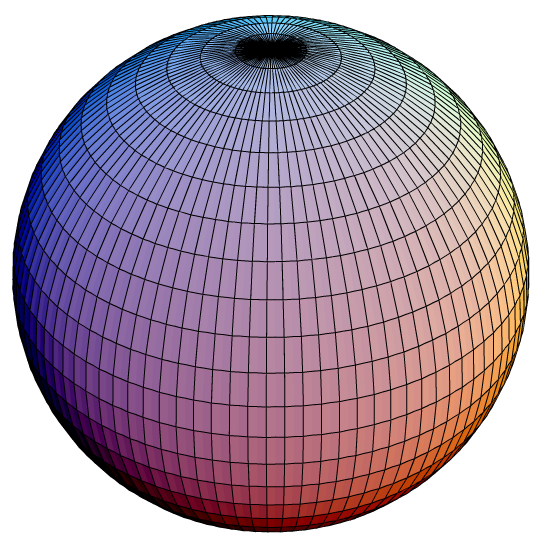
\includegraphics[scale=0.15]{manifold1.png}
						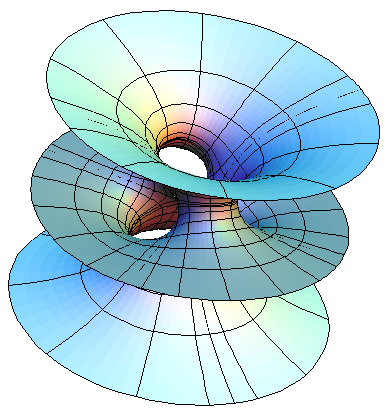
\includegraphics[scale=0.2]{manifold2.png}
						%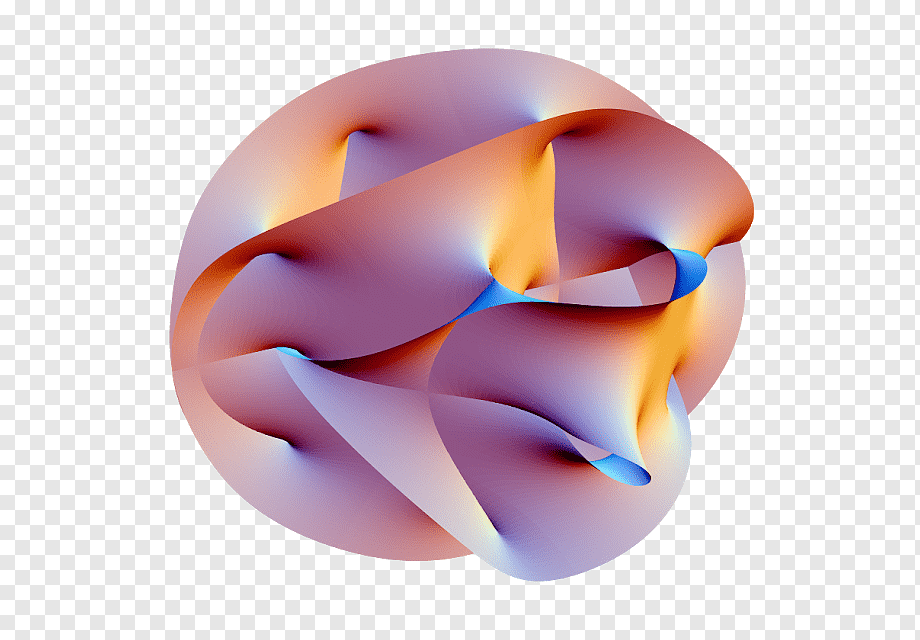
\includegraphics[scale=0.1]{manifold3.png}
						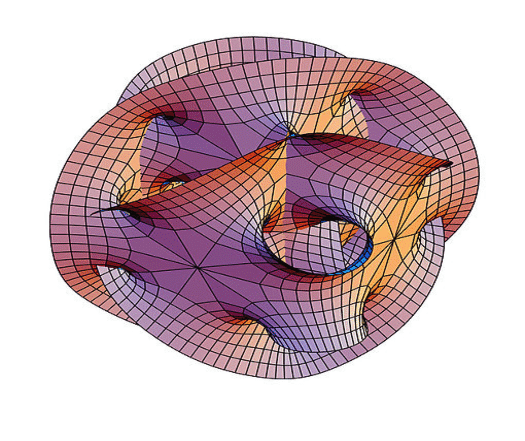
\includegraphics[scale=0.2]{manifold4.png}
				\end{figure}}}
            \end{itemize}
	\end{frame}
        \begin{frame}{Why would we care?}{}
		\begin{itemize}
            \item<1-> {A manifold is smooth means it dose not have a pointy part:\uncover<2->{\begin{figure}\centering
						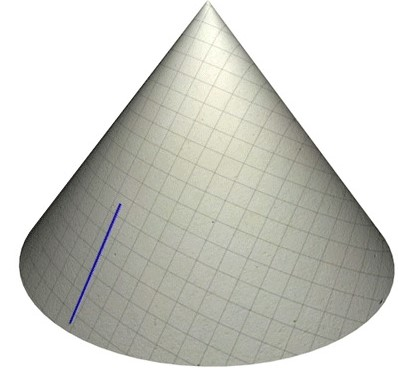
\includegraphics[scale=0.15]{singular.jpg}
				\end{figure}}}
            \item<3-> {Manifolds are also `locally Euclidean', just like the football field is flat, but the whole Earth isn't.}
            \item<4-> {When we define Yang--Mills / Instanton equations on these manifolds, the space of all solutions of these equations (we call them moduli spaces) contain a lot of topological / geometric information about the manifolds, and hence extremely lucrative to mathematicians. For similar reasons, the higher dimensional theory is extensively studied by physicists and mathematicians working on string theory and Quantum field theory.}
        \end{itemize}
	\end{frame}
	\begin{frame}%%     2
		\begin{figure}\begin{tikzpicture}[remember picture,overlay]
				% draw image
				\node[inner sep=0] at (current page.center)
				{
\includegraphics[width=\paperwidth]{thankyou.png}};
			\end{tikzpicture}
		\end{figure}
	\end{frame}
\section{code}
add more
\end{document}